\chapter{Linear Support Vector Machine}
\lecture{17}{4 Nov.}{}

\begin{prev}
    The foundations closed (\autoref{sec:power-of-three}) by naming the
    directions still open: richer transforms, smarter regularization, fewer
    labels. Two of its tools pull against each other. A feature transform
    \(\bm{\Phi}\) (\autoref{sec:nonlin-transform}) buys a sophisticated
    boundary but pays in \(\dvc\) (\autoref{sec:transform-price});
    regularization (\autoref{sec:weight-decay}) buys the complexity back by
    restricting the weights.
\end{prev}

This chapter opens the techniques half of the course, and with it topic~5:
how can machines learn by \emph{embedding numerous features}? It starts from
the plainest setting there is --- a linearly separable data set and a line
through it --- and asks which of the many separating lines to prefer. The
answer, the separating hyperplane with the largest margin, turns out to be a
quadratic program, a weight-decay regularizer and a restriction on
dichotomies all at once. That last property is what will later license
numerous features without paying for them in \(\dvc\).

\section{Course Introduction}\label{sec:mlt-intro}

\source{slides p.1--4}

\subsection{Course History}

\begin{center}
    \begin{minipage}[t]{0.47\textwidth}
        \raggedright
        \textbf{NTU Version}
        \begin{itemize}
            \item 15--17 weeks (2\(+\) hours)
            \item highly-praised with \textbf{English and blackboard
                teaching}
        \end{itemize}
        \centering
        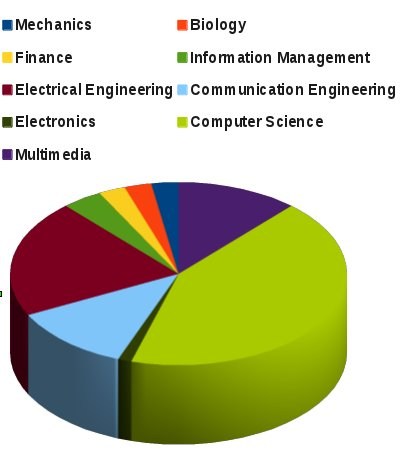
\includegraphics[width=0.62\linewidth]{Figures/ntu_ml_class_departments.jpg}
    \end{minipage}%
    \hfill
    \begin{minipage}[t]{0.47\textwidth}
        \raggedright
        \textbf{Coursera Version}
        \begin{itemize}
            \item 8 weeks of `foundations' (previous course) \(+\) 8 weeks of
                `techniques' (\textbf{this course})
            \item \textbf{Mandarin teaching} to reach more audience in need
            \item \textbf{slides teaching} improved with Coursera's quiz and
                homework mechanisms
        \end{itemize}
    \end{minipage}
\end{center}

The pie chart is the department make-up of a past NTU class: computer
science is the largest slice, electrical engineering the next, followed by
communication engineering, multimedia, information management and a few
students each from mechanics, biology, finance and electronics. The deck was
written for the Coursera split into two eight-week courses, which is why it
introduces itself as a new course; in the 2026 NTU course described in the
Preface, the two halves run in one semester, and this chapter is week~9.

\begin{moral}
    Goal: \textbf{try} making the Coursera version even better than the NTU
    version.
\end{moral}

\subsection{Course Design}

\textbf{From Foundations to Techniques}:
\begin{itemize}
    \item a mixture of philosophical illustrations, key theory, core
        algorithms, usage in practice, and hopefully jokes :-)
    \item three major techniques surrounding \textbf{feature transforms}:
        \begin{itemize}
            \item \textbf{Embedding Numerous Features}: how to exploit and
                regularize numerous features? --- inspires the
                \textbf{Support Vector Machine (SVM)} model;
            \item \textbf{Combining Predictive Features}: how to construct
                and blend predictive features? --- inspires the
                \textbf{Adaptive Boosting (AdaBoost)} model;
            \item \textbf{Distilling Implicit Features}: how to identify and
                learn implicit features? --- inspires the \textbf{Deep
                Learning} model.
        \end{itemize}
\end{itemize}

All three are answers to the question \autoref{sec:nonlin-transform} left to
the user: where does the transform \(\bm{\Phi}\) come from? There it was
hand-picked, and \autoref{sec:visual-choices} warned against picking it by
looking at the data. The three techniques take \(\bm{\Phi}\) out of human
hands in three ways --- use a huge one and control it (embed), treat each
learned hypothesis as a feature (combine), or learn the features themselves
(distill). They are topics~5, 6 and 7, the three questions
that the note at the start of Chapter~1 promised after the four of the
foundations.

\begin{moral}
    Allows students to use ML \textbf{professionally}.
\end{moral}

\begin{exercise}[Fun Time]
    Which of the following description of this course is true?
    \begin{enumerate}[(1)]
        \item the course will be taught in Taiwanese;
        \item the course will tell me the techniques that create the android
            Lieutenant Commander Data in \emph{Star Trek};
        \item the course will be 16 weeks long;
        \item the course will focus on three major techniques.
    \end{enumerate}
\end{exercise}

\begin{proof}[Reference Answer]
    (4). As for the others: (1) no, my Taiwanese is unfortunately not good
    enough for teaching (yet); (2) no, although what we teach may serve as
    building blocks; (3) no, unless you have also joined the previous course;
    (4) yes, let's get started!
\end{proof}

\subsection{Roadmap}

\begin{enumerate}
    \item \textbf{Embedding Numerous Features: Kernel Models}
        \begin{itemize}
            \item[] \textbf{Lecture 1: Linear Support Vector Machine} ---
                Course Introduction; Large-Margin Separating Hyperplane;
                Standard Large-Margin Problem; Support Vector Machine; Reasons
                behind Large-Margin Hyperplane
        \end{itemize}
    \item Combining Predictive Features: Aggregation Models
    \item Distilling Implicit Features: Extraction Models
\end{enumerate}

\section{Large-Margin Separating Hyperplane}\label{sec:large-margin}

\source{slides p.5--10}

\subsection{Linear Classification Revisited}

\begin{center}
    \begin{minipage}[c]{0.5\textwidth}
        \centering
        \textbf{PLA/pocket}\\[4pt]
        \(h(\bm{x}) = \sign(s)\)\\[4pt]
        \scoreunit{sign}\\[4pt]
        plausible \(\err = 0/1\)\\
        {\small (small flipping noise)}\\
        minimize \textbf{specially}
    \end{minipage}%
    \hfill
    \begin{minipage}[c]{0.42\textwidth}
        \centering
        \begin{tikzpicture}[scale=2.4]
            \fill[neghalf] (0,0) rectangle (1,1);
            \fill[poshalf] (0.498,1) -- (1,1) -- (1,0) -- (0.694,0) -- cycle;
            \draw[sepline] (0.498,1) -- (0.694,0);
            \foreach \p in {(0.196,0.845), (0.447,0.746), (0.347,0.323),
                    (0.546,0.100)}{\node[dneg] at \p {\(\times\)};}
            \foreach \p in {(0.670,0.797), (0.945,0.646), (0.691,0.498),
                    (0.897,0.347), (0.711,0.199)}{\node[dpos] at \p {};}
            \draw[plotbox] (0,0) rectangle (1,1);
        \end{tikzpicture}\\[2pt]
        {\small (linear separable)}
    \end{minipage}
\end{center}

This is the binary classification of the foundations, in one picture: the
perceptron scores \(\bm{x}\) linearly and takes the sign. The error measure
\(0/1\) is plausible when the noise only flips a few labels, and it has to be
minimized \emph{specially} because minimizing it in general is NP-hard ---
hence PLA (\autoref{alg:pla}) when the data are linearly separable, as on the
right, and pocket (\autoref{alg:pocket}) when they are not.

\begin{moral}
    Linear (hyperplane) classifiers: \(h(\bm{x}) = \sign(\bm{w}^\top
    \bm{x})\).
\end{moral}

\subsection{Which Line Is Best?}

\begin{question}
    Which line is best?
\end{question}

\begin{center}
    \svmtoypanel{0.3725}{-1}{-0.167}\quad
    \svmtoypanel{0.37}{-1}{-0.379}\quad
    \svmtoypanel{1}{-1}{-1}
\end{center}

The three lines separate the same four examples --- the deck's toy data set,
which \autoref{sec:svm} will solve by hand --- and nothing in the
foundations ranks them.
\begin{itemize}
    \item PLA? Depending on randomness: which of them it returns depends on
        the order in which it meets its mistakes.
    \item VC bound? Whichever you like!
        \[
            \Eout(\bm{w}) \le \underbrace{\Ein(\bm{w})}_{0} +
            \underbrace{\Omega(\mathcal{H})}_{\dvc = d + 1}
        \]
        All three have \(\Ein = 0\) and come from the same \(\mathcal{H}\),
        so the bound is identical for all of them.
\end{itemize}

\begin{moral}
    You? \textbf{Rightmost one}, possibly :-)
\end{moral}

\subsection{Why Rightmost Hyperplane?}

\begin{center}
    \svmtoypanel[disk]{0.3725}{-1}{-0.167}\quad
    \svmtoypanel[disk]{0.37}{-1}{-0.379}\quad
    \svmtoypanel[disk]{1}{-1}{-1}
\end{center}

\textbf{Informal argument}: if there is (Gaussian-like) noise on a future
\(\bm{x} \approx \bm{x}_n\),
\begin{center}
    \begin{tabular}{@{}l@{\qquad}l@{}}
        \(\bm{x}_n\) further from hyperplane & distance to closest
            \(\bm{x}_n\)\\
        \(\iff\) tolerate more noise & \(\iff\) amount of noise tolerance\\
        \(\iff\) more robust to overfitting & \(\iff\) robustness of
            hyperplane
    \end{tabular}
\end{center}

Each grey disk has radius equal to the distance from the line to the
\emph{closest} example, computed from the data, so it is the same in every
panel of a row and grows from left to right. A future input that is a noisy
copy of some \(\bm{x}_n\) and lands inside its disk is still classified like
\(\bm{x}_n\). The left column is read example by example (the further each
\(\bm{x}_n\), the more noise it survives); the right column is read for the
hyperplane as a whole, whose tolerance is set by its weakest example.
Noise is what drives overfitting (\autoref{sec:noise-data-size}), so a
hyperplane that tolerates more of it is less likely to have fitted it.

\begin{moral}
    Rightmost one: \textbf{more robust}, because of \textbf{larger distance
    to closest \(\bm{x}_n\)}.
\end{moral}

\subsection{Fat Hyperplane}

\begin{center}
    \svmtoypanel[disk]{0.3725}{-1}{-0.167}\quad
    \svmtoypanel[disk]{0.37}{-1}{-0.379}\quad
    \svmtoypanel[disk]{1}{-1}{-1}\\[6pt]
    \svmtoypanel[band]{0.3725}{-1}{-0.167}\quad
    \svmtoypanel[band]{0.37}{-1}{-0.379}\quad
    \svmtoypanel[band]{1}{-1}{-1}
\end{center}

The two rows draw the same number twice. A disk of radius \(\rho\) around
every example stays clear of the line exactly when a strip of half-width
\(\rho\) around the line stays clear of every example. The second view moves
the robustness from the data onto the hyperplane, which is what we choose.
\begin{itemize}
    \item A robust separating hyperplane is \textbf{fat}: far from both sides
        of examples.
    \item Robustness \(\equiv\) \textbf{fatness}: the distance to the closest
        \(\bm{x}_n\).
\end{itemize}

\begin{moral}
    Goal: find the \textbf{fattest} separating hyperplane.
\end{moral}

\subsection{Large-Margin Separating Hyperplane}

\begin{center}
    \svmtoypanel[band]{0.3725}{-1}{-0.167}\quad
    \svmtoypanel[band]{0.37}{-1}{-0.379}\quad
    \svmtoypanel[band]{1}{-1}{-1}
\end{center}

Written as an optimization problem, the goal reads
\[
    \begin{aligned}
        \max_{\bm{w}} \quad & \operatorname{fatness}(\bm{w})\\
        \text{subject to} \quad & \bm{w} \text{ classifies every }
            (\bm{x}_n, y_n) \text{ correctly},\\
        & \operatorname{fatness}(\bm{w}) = \min_{n=1,\dots,N}
            \operatorname{distance}(\bm{x}_n, \bm{w}).
    \end{aligned}
\]

\begin{definition}[Margin]
    The fatness of a separating hyperplane --- the distance to its closest
    example --- is formally called its \vocab{margin}.
\end{definition}

Correctness also has a formula: \(y_n = \sign(\bm{w}^\top \bm{x}_n)\), which
for the \(\pm 1\) labels is the same as \(y_n \bm{w}^\top \bm{x}_n > 0\).
Substituting both names gives
\[
    \begin{aligned}
        \max_{\bm{w}} \quad & \operatorname{margin}(\bm{w})\\
        \text{subject to} \quad & \text{every } y_n \bm{w}^\top \bm{x}_n >
            0,\\
        & \operatorname{margin}(\bm{w}) = \min_{n=1,\dots,N}
            \operatorname{distance}(\bm{x}_n, \bm{w}).
    \end{aligned}
\]

\begin{moral}
    Goal: find the \textbf{largest-margin separating} hyperplane.
\end{moral}

\begin{exercise}[Fun Time]
    Consider two examples \((\bm{v}, +1)\) and \((-\bm{v}, -1)\) where
    \(\bm{v} \in \mathbb{R}^2\) (without padding the \(v_0 = 1\)). Which of
    the following hyperplanes is the largest-margin separating one for the
    two examples? You are highly encouraged to visualize by considering, for
    instance, \(\bm{v} = (3, 2)\).
    \begin{enumerate}[(1)]
        \item \(x_1 = 0\);
        \item \(x_2 = 0\);
        \item \(v_1 x_1 + v_2 x_2 = 0\);
        \item \(v_2 x_1 + v_1 x_2 = 0\).
    \end{enumerate}
\end{exercise}

\begin{proof}[Reference Answer]
    (3). Here the largest-margin separating hyperplane (line) must be the
    perpendicular bisector of the line segment between \(\bm{v}\) and
    \(-\bm{v}\): any other separating line is closer to one of the two
    points. Hence \(\bm{v}\) is a normal vector of the largest-margin line,
    and since the midpoint is the origin, the line is \(\bm{v}^\top \bm{x} =
    0\). The result extends to the more general case of \(\bm{v} \in
    \mathbb{R}^d\).
\end{proof}

\section{Standard Large-Margin Problem}\label{sec:standard-lm}

\source{slides p.11--16}

The problem of \autoref{sec:large-margin} is stated, but not in a form any
solver accepts: \(\operatorname{distance}(\bm{x}_n, \bm{w})\) has no formula
yet, and a \(\max\) of a \(\min\) is awkward. This section turns it into a
standard problem in four steps.

\subsection{Distance to Hyperplane: Preliminary}

\[
    \begin{aligned}
        \max_{\bm{w}} \quad & \operatorname{margin}(\bm{w})\\
        \text{subject to} \quad & \text{every } y_n \bm{w}^\top \bm{x}_n >
            0,\\
        & \operatorname{margin}(\bm{w}) = \min_{n=1,\dots,N}
            \operatorname{distance}(\bm{x}_n, \bm{w}).
    \end{aligned}
\]

`Shorten' \(\bm{x}\) and \(\bm{w}\): the distance needs \(w_0\) and
\((w_1, \dots , w_d)\) differently (to be derived), so pull \(w_0\) out of
the vector.
\[
    b = w_0; \qquad
    \bm{w} = \begin{bmatrix} w_1 \\ \vdots \\ w_d \end{bmatrix}, \quad
    \bm{x} = \begin{bmatrix} x_1 \\ \vdots \\ x_d \end{bmatrix}
    \qquad (\text{the constant } x_0 = 1 \text{ is dropped}).
\]

\begin{notation}
    For this part, \(h(\bm{x}) = \sign(\bm{w}^\top \bm{x} + b)\). The vectors
    \(\bm{w}\) and \(\bm{x}\) are \(d\)-dimensional and carry no constant
    coordinate; the intercept is the separate scalar \(b\). This undoes the
    convenience of \autoref{sec:perceptron-set}, where the threshold was
    absorbed as \(w_0 x_0\).
\end{notation}

The reason is geometric: \(w_1, \dots , w_d\) give the \emph{direction} of
the hyperplane, while \(b\) only slides it along that direction. A distance
treats the two differently, so they can no longer share one vector.

\subsection{Distance to Hyperplane}

We want \(\operatorname{distance}(\bm{x}, b, \bm{w})\), with the hyperplane
\(\bm{w}^\top \bm{x}' + b = 0\).

\begin{center}
    \begin{minipage}[c]{0.56\textwidth}
        Consider \(\bm{x}'\), \(\bm{x}''\) on the hyperplane.
        \begin{enumerate}[(1)]
            \item \(\bm{w}^\top \bm{x}' = -b\), \(\bm{w}^\top \bm{x}'' =
                -b\).
            \item \(\bm{w} \perp\) hyperplane:
                \[
                    \bm{w}^\top \underbrace{(\bm{x}'' - \bm{x}')}_{
                    \text{vector on hyperplane}} = 0.
                \]
            \item distance \(=\) project \((\bm{x} - \bm{x}')\) to \(\perp\)
                hyperplane.
        \end{enumerate}
    \end{minipage}%
    \hfill
    \begin{minipage}[c]{0.4\textwidth}
        \centering
        \begin{tikzpicture}[scale=0.95, font=\small]
            \draw[black!70] (0.12,-0.70) -- (0.12,-3.20) -- (2.00,-4.20)
                -- (4.00,-3.45);
            \fill[blue!30!gray, opacity=0.55] (0.12,-2.10) -- (1.80,-2.47)
                -- (4.00,-1.98) -- (2.62,-1.60) -- cycle;
            \node[dneg] at (2.72,-2.97) {\(\times\)};
            \draw[very thick, dashed] (1.10,-0.85) -- (1.18,-2.10);
            \fill (1.18,-2.10) circle (1.6pt);
            \node[left, font=\scriptsize] at (1.12,-1.45)
                {\(\operatorname{dist}(\bm{x}, h)\)};
            \draw[very thick] (1.10,-0.85) -- (2.36,-2.20);
            \draw[black!60] (2.36,-2.20) -- (2.60,-1.73);
            \fill (2.36,-2.20) circle (1.6pt);
            \fill (2.60,-1.73) circle (1.6pt);
            \node[below right, text=orange, inner sep=1pt] at (2.36,-2.20)
                {\(\bm{x}'\)};
            \node[right, text=Purple, inner sep=5pt] at (2.60,-1.73)
                {\(\bm{x}''\)};
            \draw[-{Stealth[length=2mm]}, thick] (2.45,-1.97) -- (2.45,-1.25)
                node[above, text=blue] {\(\bm{w}\)};
            \node[dpos, minimum size=6pt, thick] at (1.10,-0.85) {};
            \node[above left, inner sep=2pt] at (1.10,-0.85) {\(\bm{x}\)};
        \end{tikzpicture}
    \end{minipage}
\end{center}

The picture is in three dimensions: the shaded sheet is the hyperplane, and
\(\bm{x}\) sits above it. Step~(2) says that \(\bm{w}\) is orthogonal to
every direction lying in the sheet, i.e.\ it is a normal vector. The
distance from \(\bm{x}\) to the sheet is then the length of the piece of
\(\bm{x} - \bm{x}'\) along that normal, for any foot point \(\bm{x}'\) on the
sheet (the solid segment), which the unit vector \(\bm{w}/\norm{\bm{w}}\)
picks out:
\[
    \operatorname{distance}(\bm{x}, b, \bm{w})
    = \abs{\frac{\bm{w}^\top}{\norm{\bm{w}}} (\bm{x} - \bm{x}')}
    \overset{(1)}{=} \frac{1}{\norm{\bm{w}}} \abs{\bm{w}^\top \bm{x} + b}.
\]
Step~(1) is what removes \(\bm{x}'\): \(\bm{w}^\top \bm{x}' = -b\) for every
point of the hyperplane, so the choice of foot point never mattered.

\subsection{Distance to Separating Hyperplane}

\[
    \operatorname{distance}(\bm{x}, b, \bm{w}) = \frac{1}{\norm{\bm{w}}}
    \abs{\bm{w}^\top \bm{x} + b}
\]
\begin{itemize}
    \item Separating hyperplane: for every \(n\),
        \[
            y_n (\bm{w}^\top \bm{x}_n + b) > 0.
        \]
    \item Distance to a separating hyperplane:
        \[
            \operatorname{distance}(\bm{x}_n, b, \bm{w}) =
            \frac{1}{\norm{\bm{w}}} y_n (\bm{w}^\top \bm{x}_n + b).
        \]
\end{itemize}
On a separating hyperplane the sign of \(\bm{w}^\top \bm{x}_n + b\) is
\(y_n\), so multiplying by \(y_n\) is the same as taking the absolute value,
and the awkward \(\abs{\cdot}\) disappears:
\begin{equation}\label{eq:lm-margin}
    \begin{aligned}
        \max_{b, \bm{w}} \quad & \operatorname{margin}(b, \bm{w})\\
        \text{subject to} \quad & \text{every } y_n (\bm{w}^\top \bm{x}_n +
            b) > 0,\\
        & \operatorname{margin}(b, \bm{w}) = \min_{n=1,\dots,N}
            \frac{1}{\norm{\bm{w}}} y_n (\bm{w}^\top \bm{x}_n + b).
    \end{aligned}
\end{equation}

\subsection{Margin of Special Separating Hyperplane}

\begin{itemize}
    \item \(\bm{w}^\top \bm{x} + b = 0\) is the same hyperplane as
        \(3\bm{w}^\top \bm{x} + 3b = 0\): scaling does not matter.
    \item Special scaling: only consider separating \((b, \bm{w})\) such
        that
        \[
            \min_{n=1,\dots,N} y_n (\bm{w}^\top \bm{x}_n + b) = 1
            \implies \operatorname{margin}(b, \bm{w}) =
            \frac{1}{\norm{\bm{w}}}.
        \]
\end{itemize}
Every hyperplane is described by a whole ray of parameter vectors \(c \cdot
(b, \bm{w})\), \(c > 0\), all with the same margin. Picking the one
representative on each ray whose closest example scores exactly \(1\)
loses no hyperplane, and it makes the \(\min\) inside the margin a constant.
\begin{equation}\label{eq:lm-scaled}
    \begin{aligned}
        \max_{b, \bm{w}} \quad & \frac{1}{\norm{\bm{w}}}\\
        \text{subject to} \quad & \text{every } y_n (\bm{w}^\top \bm{x}_n +
            b) > 0,\\
        & \min_{n=1,\dots,N} y_n (\bm{w}^\top \bm{x}_n + b) = 1.
    \end{aligned}
\end{equation}

\begin{lemma}\label{lem:special-scaling}
    \eqref{eq:lm-margin} and \eqref{eq:lm-scaled} have the same solutions
    up to positive scaling:
    \begin{enumerate}[(i)]
        \item every solution of \eqref{eq:lm-scaled} solves
            \eqref{eq:lm-margin};
        \item if \((b_1, \bm{w}_1)\) solves \eqref{eq:lm-margin} and \(s_1 =
            \min_n y_n (\bm{w}_1^\top \bm{x}_n + b_1)\), then \(\frac{1}{s_1}
            (b_1, \bm{w}_1)\) solves \eqref{eq:lm-scaled}.
    \end{enumerate}
\end{lemma}

\begin{proof}
    Let \(F_1\) and \(F_2\) be the feasible sets of \eqref{eq:lm-margin} and
    \eqref{eq:lm-scaled}. Two facts do all the work.
    \begin{itemize}
        \item \(\operatorname{margin}(cb, c\bm{w}) = \operatorname{margin}(b,
            \bm{w})\) for every \(c > 0\), since \(c\) cancels between
            \(y_n (\bm{w}^\top \bm{x}_n + b)\) and \(\norm{\bm{w}}\).
        \item \(F_2 \subseteq F_1\), and on \(F_2\) the inner \(\min\)
            equals \(1\), so \(\operatorname{margin}(b, \bm{w}) =
            \frac{1}{\norm{\bm{w}}}\) there.
    \end{itemize}
    Moreover, every \((b, \bm{w}) \in F_1\) has \(s = \min_n y_n
    (\bm{w}^\top \bm{x}_n + b) > 0\), and \(\frac{1}{s} (b, \bm{w}) \in
    F_2\).

    (i) Let \((b_2, \bm{w}_2)\) solve \eqref{eq:lm-scaled} and take any
    \((b, \bm{w}) \in F_1\). With \(s\) as above,
    \[
        \operatorname{margin}(b, \bm{w}) =
        \operatorname{margin}\left( \tfrac{1}{s} (b, \bm{w}) \right) =
        \frac{1}{\norm{\bm{w} / s}} \le \frac{1}{\norm{\bm{w}_2}} =
        \operatorname{margin}(b_2, \bm{w}_2),
    \]
    the inequality because \(\frac{1}{s} (b, \bm{w}) \in F_2\) and \((b_2,
    \bm{w}_2)\) is optimal there. So \((b_2, \bm{w}_2) \in F_1\) is at least
    as good as every point of \(F_1\).

    (ii) \(\frac{1}{s_1} (b_1, \bm{w}_1) \in F_2\), and for any \((b, \bm{w})
    \in F_2 \subseteq F_1\),
    \[
        \frac{1}{\norm{\bm{w}}} = \operatorname{margin}(b, \bm{w}) \le
        \operatorname{margin}(b_1, \bm{w}_1) =
        \operatorname{margin}\left( \tfrac{1}{s_1} (b_1, \bm{w}_1) \right) =
        \frac{1}{\norm{\bm{w}_1 / s_1}},
    \]
    the inequality because \((b_1, \bm{w}_1)\) is optimal in \(F_1\). So
    \(\frac{1}{s_1} (b_1, \bm{w}_1)\) is at least as good as every point of
    \(F_2\).
\end{proof}

The first constraint is now implied by the second, so it can go.

\subsection{Standard Large-Margin Hyperplane Problem}

\[
    \max_{b, \bm{w}} \ \frac{1}{\norm{\bm{w}}} \quad \text{subject to}
    \quad \min_{n=1,\dots,N} y_n (\bm{w}^\top \bm{x}_n + b) = 1
\]
A \(\min\) inside a constraint is still not standard. Its \emph{necessary}
consequence is a set of plain inequalities: \(y_n (\bm{w}^\top \bm{x}_n + b)
\ge 1\) for all \(n\). Relaxing to those is safe.

\begin{lemma}
    Replacing the constraint \(\min_n y_n (\bm{w}^\top \bm{x}_n + b) = 1\)
    by \(y_n (\bm{w}^\top \bm{x}_n + b) \ge 1\) for all \(n\) does not change
    the optimal \((b, \bm{w})\).
\end{lemma}

\begin{proof}
    The relaxed feasible set contains the original one, so it suffices to
    show the relaxed optimum lies inside the original set. Suppose it does
    not: then the optimal \((b, \bm{w})\) is outside, e.g.\ \(y_n
    (\bm{w}^\top \bm{x}_n + b) > 1.126\) for all \(n\). Then we can scale
    \((b, \bm{w})\) to the ``more optimal'' \(\left( \frac{b}{1.126},
    \frac{\bm{w}}{1.126} \right)\), which still satisfies every \(\ge 1\)
    constraint and has a larger \(\frac{1}{\norm{\bm{w}}}\) --- a
    contradiction.
\end{proof}

Final change: \(\max \implies \min\), remove the \(\sqrt{\phantom{x}}\), add
\(\frac{1}{2}\). Maximizing \(\frac{1}{\norm{\bm{w}}}\) is minimizing
\(\norm{\bm{w}}\); squaring and halving it moves no minimizer and leaves a
quadratic with a clean gradient.

\begin{moral}
    \[
        \begin{aligned}
            \min_{b, \bm{w}} \quad & \frac{1}{2} \bm{w}^\top \bm{w}\\
            \text{subject to} \quad & y_n (\bm{w}^\top \bm{x}_n + b) \ge 1
                \text{ for all } n.
        \end{aligned}
    \]
\end{moral}

\begin{exercise}[Fun Time]
    Consider three examples \((\bm{x}_1, +1)\), \((\bm{x}_2, +1)\),
    \((\bm{x}_3, -1)\), where \(\bm{x}_1 = (3, 0)\), \(\bm{x}_2 = (0, 4)\),
    \(\bm{x}_3 = (0, 0)\). In addition, consider a hyperplane \(x_1 + x_2 =
    1\). Which of the following is \textbf{not} true?
    \begin{enumerate}[(1)]
        \item the hyperplane is a separating one for the three examples;
        \item the distance from the hyperplane to \(\bm{x}_1\) is \(2\);
        \item the distance from the hyperplane to \(\bm{x}_3\) is
            \(\frac{1}{\sqrt{2}}\);
        \item the example that is closest to the hyperplane is \(\bm{x}_3\).
    \end{enumerate}
\end{exercise}

\begin{proof}[Reference Answer]
    (2). With \(\bm{w} = (1, 1)\) and \(b = -1\), the distance from the
    hyperplane to \(\bm{x}_1\) is \(\frac{1}{\sqrt{2}} (3 + 0 - 1) =
    \sqrt{2}\). (The other three hold: the scores \(y_n(\bm{w}^\top \bm{x}_n
    + b)\) are \(2, 3, 1\), all positive, giving distances \(\sqrt{2},
    \frac{3}{\sqrt{2}}, \frac{1}{\sqrt{2}}\).)
\end{proof}

\section{Support Vector Machine}\label{sec:svm}

\source{slides p.17--22}

\subsection{Solving a Particular Standard Problem}

Before reaching for a solver, solve the standard problem
\[
    \min_{b, \bm{w}} \ \frac{1}{2} \bm{w}^\top \bm{w} \quad \text{subject
    to} \quad y_n (\bm{w}^\top \bm{x}_n + b) \ge 1 \text{ for all } n
\]
on the four examples of \autoref{sec:large-margin} by hand.

\begin{center}
    \begin{minipage}[c]{0.66\textwidth}
        \[
            \mathrm{X} = \begin{bmatrix} 0 & 0 \\ 2 & 2 \\ 2 & 0 \\ 3 & 0
            \end{bmatrix}, \quad
            \bm{y} = \begin{bmatrix} -1 \\ -1 \\ +1 \\ +1 \end{bmatrix}
            \qquad
            \begin{aligned}
                -b &\ge 1 & \text{(i)}\\
                -2w_1 - 2w_2 - b &\ge 1 & \text{(ii)}\\
                2w_1 + b &\ge 1 & \text{(iii)}\\
                3w_1 + b &\ge 1 & \text{(iv)}
            \end{aligned}
        \]
    \end{minipage}%
    \hfill
    \begin{minipage}[c]{0.3\textwidth}
        \centering
        \svmtoypanel[band]{1}{-1}{-1}
    \end{minipage}
\end{center}

\begin{itemize}
    \item \(\left\{ \begin{aligned}
            \text{(i)} \ \& \ \text{(iii)} &\implies w_1 \ge +1\\
            \text{(ii)} \ \& \ \text{(iii)} &\implies w_2 \le -1
        \end{aligned} \right\} \implies \frac{1}{2} \bm{w}^\top \bm{w} \ge
        1\).

        Adding (i) and (iii) gives \(2w_1 \ge 2\); adding (ii) and (iii)
        gives \(-2w_2 \ge 2\). So \(w_1^2 \ge 1\) and \(w_2^2 \ge 1\), and the
        objective \(\frac{1}{2}(w_1^2 + w_2^2)\) is at least \(1\).
    \item \((w_1 = 1, w_2 = -1, b = -1)\) is at the \textbf{lower bound} and
        satisfies (i)--(iv): the four constraints read \(1 \ge 1\), \(1 \ge
        1\), \(1 \ge 1\), \(2 \ge 1\). A feasible point attaining a lower
        bound is optimal.
\end{itemize}

\begin{moral}
    \(g_{\mathrm{SVM}}(\bm{x}) = \sign(x_1 - x_2 - 1)\): SVM? :-)
\end{moral}

\subsection{Support Vector Machine (SVM)}

\begin{center}
    \begin{minipage}[c]{0.56\textwidth}
        \begin{tabular}{@{}ll@{}}
            optimal solution: & \((w_1 = 1, w_2 = -1, b = -1)\)\\[4pt]
            \(\operatorname{margin}(b, \bm{w})\) & \(=
                \dfrac{1}{\norm{\bm{w}}} = \dfrac{1}{\sqrt{2}}\)
        \end{tabular}
    \end{minipage}%
    \hfill
    \begin{minipage}[c]{0.4\textwidth}
        \centering
        \svmtoysolution
    \end{minipage}
\end{center}

The grey strip has half-width \(\frac{1}{\sqrt{2}} \approx 0.707\), and its
two edges are the lines \(x_1 - x_2 - 1 = \pm 1\), where the special
scaling makes \(y_n(\bm{w}^\top \bm{x}_n + b)\) exactly \(1\). Three
examples (boxed) sit on those edges; the fourth, \((3, 0)\), is strictly
outside.
\begin{itemize}
    \item Examples on the boundary `locate' the fattest hyperplane, and
        the other examples are \textbf{not needed}. Deleting \((3, 0)\) would leave
        only constraints (i)--(iii), with the same solution.
    \item Call a boundary example a \vocab{support vector} (candidate).
\end{itemize}
The word ``candidate'' is deliberate: being on the boundary is necessary for
an example to matter, and the precise definition is left for the next
chapter.

\begin{moral}
    \textbf{Support vector machine (SVM)}: learn the \textbf{fattest
    hyperplanes} (with the help of \textbf{support vectors}).
\end{moral}

\subsection{Solving General SVM}

\[
    \min_{b, \bm{w}} \ \frac{1}{2} \bm{w}^\top \bm{w} \quad \text{subject
    to} \quad y_n (\bm{w}^\top \bm{x}_n + b) \ge 1 \text{ for all } n
\]
\begin{itemize}
    \item Not easy manually, of course :-)
    \item Gradient descent? Not easy with constraints: a step downhill may
        leave the feasible set, and nothing in the update brings it back.
    \item Luckily:
        \begin{itemize}
            \item a (convex) \textbf{quadratic} objective function of \((b,
                \bm{w})\);
            \item \textbf{linear} constraints of \((b, \bm{w})\)
        \end{itemize}
        --- this is \vocab{quadratic programming}.
\end{itemize}

\begin{moral}
    Quadratic programming (QP): an `easy' optimization problem.
\end{moral}

`Easy' here means that the problem class is well understood and solved
reliably by off-the-shelf solvers, so all that remains is to hand them the
SVM in their own format.

\subsection{Quadratic Programming}

\begin{center}
    \begin{tabular}{@{}c@{\qquad}c@{}}
        optimal \((b, \bm{w}) = \ ?\) & optimal \(\bm{u} \gets
            \mathrm{QP}(\mathrm{Q}, \bm{p}, \mathrm{A}, \bm{c})\)\\[6pt]
        \(\begin{aligned}
            \min_{b, \bm{w}} \quad & \tfrac{1}{2} \bm{w}^\top \bm{w}\\
            \text{subject to} \quad & y_n (\bm{w}^\top \bm{x}_n + b) \ge 1,\\
            & \text{for } n = 1, 2, \dots , N
        \end{aligned}\)
        &
        \(\begin{aligned}
            \min_{\bm{u}} \quad & \tfrac{1}{2} \bm{u}^\top \mathrm{Q} \bm{u}
                + \bm{p}^\top \bm{u}\\
            \text{subject to} \quad & \bm{a}_m^\top \bm{u} \ge c_m,\\
            & \text{for } m = 1, 2, \dots , M
        \end{aligned}\)
    \end{tabular}
\end{center}

Matching the two term by term:
\[
    \text{objective function:} \quad
    \bm{u} = \begin{bmatrix} b \\ \bm{w} \end{bmatrix}; \quad
    \mathrm{Q} = \begin{bmatrix} 0 & \bm{0}_d^\top \\ \bm{0}_d &
    \mathrm{I}_d \end{bmatrix}; \quad
    \bm{p} = \bm{0}_{d+1}
\]
\[
    \text{constraints:} \quad
    \bm{a}_n^\top = y_n \begin{bmatrix} 1 & \bm{x}_n^\top \end{bmatrix};
    \quad c_n = 1; \quad M = N
\]
The zero corner of \(\mathrm{Q}\) is the price of separating \(b\) from
\(\bm{w}\): \(\frac{1}{2} \bm{u}^\top \mathrm{Q} \bm{u} = \frac{1}{2}
\bm{w}^\top \bm{w}\), so the intercept is free and only the direction is
penalized. Each example contributes one row \(\bm{a}_n^\top\), and
\(\bm{a}_n^\top \bm{u} = y_n (b + \bm{w}^\top \bm{x}_n)\) is exactly its
constraint.

\begin{moral}
    SVM with a general QP solver: easy if you've read the manual :-)
\end{moral}

\subsection{SVM with QP Solver}

\begin{algorithm}[H]
    \caption{Linear Hard-Margin SVM}\label{alg:linear-hard-svm}
    \KwIn{linearly separable
        \(\mathcal{D} = \left\{ (\bm{x}_n, y_n) \right\}_{n=1}^{N}\)}
    \KwOut{\(b\) and \(\bm{w}\), returned as \(g_{\mathrm{SVM}}\)}
    \(\mathrm{Q} = \begin{bmatrix} 0 & \bm{0}_d^\top \\ \bm{0}_d &
        \mathrm{I}_d \end{bmatrix}\); \(\bm{p} = \bm{0}_{d+1}\);
        \(\bm{a}_n^\top = y_n \begin{bmatrix} 1 & \bm{x}_n^\top
        \end{bmatrix}\); \(c_n = 1\)\;
    \(\begin{bmatrix} b \\ \bm{w} \end{bmatrix} \gets
        \mathrm{QP}(\mathrm{Q}, \bm{p}, \mathrm{A}, \bm{c})\)\;
    \Return \(b\) \& \(\bm{w}\) as \(g_{\mathrm{SVM}}\)\;
\end{algorithm}

\begin{itemize}
    \item \textbf{Hard-margin}: nothing violates the `fat boundary' --- every
        constraint must hold, so the data must be linearly separable.
    \item \textbf{Linear}: the inputs are the raw \(\bm{x}_n\).
\end{itemize}

\begin{question}
    Want non-linear?
\end{question}

\(\bm{z}_n = \bm{\Phi}(\bm{x}_n)\) --- remember? :-) Feed the transformed
inputs to \autoref{alg:linear-hard-svm} exactly as
\autoref{alg:feature-transform} fed them to any linear model. The catch is
the size of the QP: it has \(\tilde{d} + 1\) variables, which is what the
next chapters will work around.

\begin{exercise}[Fun Time]
    Consider two negative examples with \(\bm{x}_1 = (0, 0)\) and \(\bm{x}_2
    = (2, 2)\); two positive examples with \(\bm{x}_3 = (2, 0)\) and
    \(\bm{x}_4 = (3, 0)\), as shown on page~17 of the slides. Define
    \(\bm{u}\), \(\mathrm{Q}\), \(\bm{p}\), \(c_n\) as those listed on
    page~20 of the slides. What are the \(\bm{a}_n^\top\) that need to be fed
    into the QP solver?
    \begin{enumerate}[(1)]
        \item \(\bm{a}_1^\top = [-1, 0, 0]\), \(\bm{a}_2^\top = [-1, 2,
            2]\), \(\bm{a}_3^\top = [-1, 2, 0]\), \(\bm{a}_4^\top = [-1, 3,
            0]\);
        \item \(\bm{a}_1^\top = [1, 0, 0]\), \(\bm{a}_2^\top = [1, -2,
            -2]\), \(\bm{a}_3^\top = [-1, 2, 0]\), \(\bm{a}_4^\top = [-1, 3,
            0]\);
        \item \(\bm{a}_1^\top = [1, 0, 0]\), \(\bm{a}_2^\top = [1, 2, 2]\),
            \(\bm{a}_3^\top = [1, 2, 0]\), \(\bm{a}_4^\top = [1, 3, 0]\);
        \item \(\bm{a}_1^\top = [-1, 0, 0]\), \(\bm{a}_2^\top = [-1, -2,
            -2]\), \(\bm{a}_3^\top = [1, 2, 0]\), \(\bm{a}_4^\top = [1, 3,
            0]\).
    \end{enumerate}
\end{exercise}

\begin{proof}[Reference Answer]
    (4). We need \(\bm{a}_n^\top = y_n \begin{bmatrix} 1 & \bm{x}_n^\top
    \end{bmatrix}\): the whole row, constant \(1\) included, is multiplied by
    the label. These four rows are the left-hand sides of constraints
    (i)--(iv) above.
\end{proof}

\section{Reasons behind Large-Margin Hyperplane}\label{sec:why-large-margin}

\source{slides p.23--27}

The large-margin hyperplane was motivated by an informal story about noise.
This section gives two reasons in the language of the foundations: it is a
regularizer, and it has a smaller effective VC dimension.

\subsection{Why Large-Margin Hyperplane?}

\[
    \min_{b, \bm{w}} \ \frac{1}{2} \bm{w}^\top \bm{w} \quad \text{subject
    to} \quad y_n (\bm{w}^\top \bm{z}_n + b) \ge 1 \text{ for all } n
\]

\begin{center}
    \solidrules
    \begin{tabular}{l|c|c}
        \toprule
        & minimize & constraint\\
        \midrule
        regularization & \(\Ein\) & \(\bm{w}^\top \bm{w} \le C\)\\
        SVM & \(\bm{w}^\top \bm{w}\) & \(\Ein = 0\) [and more]\\
        \bottomrule
    \end{tabular}
\end{center}

The two problems hold the same pair of quantities with the roles swapped.
Weight decay (\autoref{def:weight-decay}) minimizes the error inside a
budget on \(\bm{w}^\top \bm{w}\); the SVM minimizes \(\bm{w}^\top \bm{w}\)
among the hyperplanes with zero error. ``And more'' because the constraint
\(y_n(\bm{w}^\top \bm{z}_n + b) \ge 1\) asks not just for the right side but
for a score of at least \(1\).

\begin{moral}
    SVM (large-margin hyperplane): `weight-decay regularization' within
    \(\Ein = 0\).
\end{moral}

\subsection{Large-Margin Restricts Dichotomies}

Consider the `large-margin algorithm' \(\mathcal{A}_\rho\): it either
\textbf{returns \(g\) with \(\operatorname{margin}(g) \ge \rho\) (if one
exists)}, or \(0\) otherwise.

\textbf{\(\mathcal{A}_0\)}: like PLA \(\implies\) shatter `general' 3 inputs.
\begin{center}
    \begin{tikzpicture}[scale=1.9]
        \draw[sepline] (0,0.34) -- (0.66,1);
        \draw[plotbox] (0,0) rectangle (1,1);
        \arhodata{o}{o}{o}
        \begin{scope}[xshift=1.3cm]
            \draw[sepline] (0,0.63) -- (1,0.14);
            \draw[plotbox] (0,0) rectangle (1,1);
            \arhodata{x}{o}{o}
        \end{scope}
        \begin{scope}[xshift=2.6cm]
            \draw[sepline] (0,0.32) -- (1,0.82);
            \draw[plotbox] (0,0) rectangle (1,1);
            \arhodata{o}{x}{o}
        \end{scope}
        \begin{scope}[xshift=3.9cm]
            \draw[sepline] (0.23,0) -- (1,0.76);
            \draw[plotbox] (0,0) rectangle (1,1);
            \arhodata{x}{x}{o}
        \end{scope}
    \end{tikzpicture}
\end{center}

\textbf{\(\mathcal{A}_{1.126}\)}: more strict than SVM \(\implies\) cannot
shatter any 3 inputs.
\begin{center}
    \begin{tikzpicture}[scale=1.9]
        \begin{scope}
            \clip (0,0) rectangle (1,1);
            \fill[fatband] (-1.588,-2.150) -- (1.379,3.065) -- (1.814,2.817)
                -- (-1.154,-2.397) -- cycle;
            \draw[sepline] (-1.371,-2.274) -- (1.596,2.941);
        \end{scope}
        \draw[{Stealth[length=1.2mm]}-{Stealth[length=1.2mm]}, thin]
            (0.113,0.334) -- (0.330,0.210);
        \node[font=\tiny, above right, inner sep=0.5pt] at (0.20,0.29)
            {\(\rho\)};
        \draw[plotbox] (0,0) rectangle (1,1);
        \arhodata{o}{o}{o}
        \begin{scope}[xshift=1.3cm]
            \begin{scope}
                \clip (0,0) rectangle (1,1);
                \fill[fatband] (-0.891,3.358) -- (2.144,-1.818)
                    -- (1.712,-2.071) -- (-1.322,3.106) -- cycle;
                \draw[sepline] (-1.106,3.232) -- (1.928,-1.944);
            \end{scope}
            \draw[plotbox] (0,0) rectangle (1,1);
            \arhodata{x}{o}{o}
        \end{scope}
        \begin{scope}[xshift=2.6cm]
            \begin{scope}
                \clip (0,0) rectangle (1,1);
                \fill[fatband] (-2.475,-0.934) -- (2.715,2.077)
                    -- (2.966,1.644) -- (-2.224,-1.366) -- cycle;
                \draw[fatedge] (-2.475,-0.934) -- (2.715,2.077);
                \draw[fatedge] (-2.224,-1.366) -- (2.966,1.644);
                \draw[fatcore] (-2.349,-1.150) -- (2.841,1.861);
            \end{scope}
            \draw[plotbox] (0,0) rectangle (1,1);
            \arhodata[faint]{o}{x}{o}
        \end{scope}
        \begin{scope}[xshift=3.9cm]
            \begin{scope}
                \clip (0,0) rectangle (1,1);
                \fill[fatband] (-1.244,-2.346) -- (1.723,2.869)
                    -- (2.157,2.622) -- (-0.810,-2.593) -- cycle;
                \draw[fatedge] (-1.244,-2.346) -- (1.723,2.869);
                \draw[fatedge] (-0.810,-2.593) -- (2.157,2.622);
                \draw[fatcore] (-1.027,-2.469) -- (1.940,2.745);
            \end{scope}
            \draw[plotbox] (0,0) rectangle (1,1);
            \arhodata[faint]{x}{x}{o}
        \end{scope}
    \end{tikzpicture}
\end{center}

The four panels of each row are four of the eight dichotomies of the same
three inputs; the remaining four are their label flips, handled by the same
lines. With \(\rho = 0\) any separating line will do, so \(\mathcal{A}_0\)
produces all eight, just like a perceptron. With a large \(\rho\), a
dichotomy survives only if a strip of half-width \(\rho\) fits between its
two classes. In the redraw (my measurements: the square is the unit square
and \(\rho = 0.25\)), the best strips of the four dichotomies have half-widths
\(\infty\), \(0.289\), \(0.168\) and \(0.146\). The first two exceed \(\rho\);
the last two do not, so even their best strip, drawn faded with its dashed
edges, swallows the inputs, and \(\mathcal{A}_\rho\) returns \(0\). The deck
writes the strict algorithm as \(\mathcal{A}_{1.126}\); the number only has to
exceed what those dichotomies can offer.

\begin{moral}
    Fewer dichotomies \(\implies\) smaller `VC dim.' \(\implies\)
    \textbf{better generalization}.
\end{moral}

\subsection{VC Dimension of Large-Margin Algorithm}

Fewer dichotomies \(\implies\) smaller `VC dim.', but the quantity here is a
new one:
\begin{itemize}
    \item it considers \(\dvc(\mathcal{A}_\rho)\) [\textbf{data-dependent},
        need more than VC]
    \item instead of \(\dvc(\mathcal{H})\) [data-independent, covered by VC].
\end{itemize}
\begin{remark}[\(\dvc\) of an algorithm]
    \autoref{def:vc} measures a \emph{set}: \(\mathcal{H}\) shatters
    \(\bm{x}_1, \dots, \bm{x}_N\) when each of the \(2^N\) labellings is
    realized by some \(h \in \mathcal{H}\), and \(\dvc(\mathcal{H})\) is the
    most inputs it can shatter. An algorithm is not a set, so the count is
    rephrased through its output. Hand \(\mathcal{A}_\rho\) the inputs
    together with a labelling \(y_1, \dots, y_N\): the labelling is
    \emph{produced} if \(\mathcal{A}_\rho\) returns a hyperplane classifying
    every \(\bm{x}_n\) as \(y_n\), and not produced if it gives up and returns
    \(0\). \(\mathcal{A}_\rho\) shatters the inputs when it produces all
    \(2^N\) labellings, and \(\dvc(\mathcal{A}_\rho)\) is the most inputs in
    \(\mathcal{X}\) it can shatter --- exactly what the two rows of panels
    above counted.

    The difference from \(\mathcal{H}\): whether a labelling is produced
    depends on how far apart the inputs are, because the margin does. That is
    the sense of ``data-dependent''. It is also why \(\mathcal{X}\) is bounded
    below: on all of \(\mathbb{R}^d\) the inputs could be spread out until
    every labelling clears \(\rho\), and \(\dvc(\mathcal{A}_\rho)\) would be
    \(d + 1\) again.
\end{remark}

\begin{center}
    \begin{minipage}[c]{0.66\textwidth}
        \(\dvc(\mathcal{A}_\rho)\) when \(\mathcal{X} =\) unit circle in
        \(\mathbb{R}^2\):
        \begin{itemize}
            \item \(\rho = 0\): just perceptrons (\(\dvc = 3\));
            \item \(\rho > \frac{\sqrt{3}}{2}\): cannot shatter any 3 inputs
                (\(\dvc < 3\)) --- some inputs must be of \textbf{distance
                \(\le \sqrt{3}\)}.
        \end{itemize}
    \end{minipage}%
    \hfill
    \begin{minipage}[c]{0.3\textwidth}
        \centering
        \begin{tikzpicture}[scale=0.9]
            \fill[ForestGreen!45] (0,0) circle (1);
            \draw[ForestGreen!70!black] (0,0) circle (1);
            \node[dneg] at (67:1) {\(\times\)};
            \node[dpos, fill=white] at (0:1) {};
            \node[dneg] at (-81:1) {\(\times\)};
        \end{tikzpicture}
    \end{minipage}
\end{center}

\begin{proof}[Why \(\sqrt{3}\)]
    Place any three inputs on the unit circle. Their three arcs add up to
    \(360^\circ\), so one arc is at most \(120^\circ\), and the chord across
    it has length at most \(2 \sin 60^\circ = \sqrt{3}\). Label those two
    inputs oppositely: any line separating them crosses the chord, so one of
    the two is within half the chord of the line, and the margin is at most
    \(\frac{\sqrt{3}}{2}\). When \(\rho > \frac{\sqrt{3}}{2}\) this dichotomy
    is out of reach.
\end{proof}

\begin{moral}
    Generally, when \(\mathcal{X}\) is in a radius-\(R\) hyperball:
    \[
        \dvc(\mathcal{A}_\rho) \le \min \left( \frac{R^2}{\rho^2}, d \right)
        + 1 \le \underbrace{d + 1}_{\dvc(\text{perceptrons})}.
    \]
\end{moral}

The bound compares the size of the input space with the width of the strip
that has to fit in it. When \(R/\rho\) is small it caps the effective
dimension no matter how large \(d\) is, which is the property needed for
the numerous features to come.

\subsection{Benefits of Large-Margin Hyperplanes}

\begin{center}
    \solidrules
    \begin{tabular}{c|c|c|c}
        \toprule
        & large-margin hyperplanes & hyperplanes & hyperplanes \(+\) feature
            transform \(\bm{\Phi}\)\\
        \midrule
        \# & even fewer & \textbf{not many} & many\\
        boundary & simple & simple & \textbf{sophisticated}\\
        \bottomrule
    \end{tabular}
\end{center}

\begin{itemize}
    \item \textbf{Not many} is good, for \(\dvc\) and generalization.
    \item \textbf{Sophisticated} is good, for possibly better \(\Ein\).
\end{itemize}

No column has both. Plain hyperplanes are few but simple; a feature
transform makes them sophisticated but many, which is the trade-off of
\autoref{sec:transform-price}. Large margins move in the opposite direction
from the transform, so combining the two might keep the good half of each.

\begin{moral}
    A new possibility: \textbf{non-linear SVM}.
    \begin{center}
        \solidrules
        \begin{tabular}{c|c}
            \toprule
            & large-margin hyperplanes \(+\) numerous feature transform
                \(\bm{\Phi}\)\\
            \midrule
            \# & \textbf{not many}\\
            boundary & \textbf{sophisticated}\\
            \bottomrule
        \end{tabular}
    \end{center}
\end{moral}

\begin{exercise}[Fun Time]
    Consider running the `large-margin algorithm' \(\mathcal{A}_\rho\) with
    \(\rho = \frac{1}{4}\) on a \(\mathcal{Z}\)-space such that \(\bm{z} =
    \bm{\Phi}(\bm{x})\) is of \(1126\) dimensions (excluding \(z_0\)) and
    \(\norm{\bm{z}} \le 1\). What is the upper bound of
    \(\dvc(\mathcal{A}_\rho)\) when calculated by \(\min \left(
    \frac{R^2}{\rho^2}, d \right) + 1\)?
    \begin{enumerate}[(1)]
        \item \(5\);
        \item \(17\);
        \item \(1126\);
        \item \(1127\).
    \end{enumerate}
\end{exercise}

\begin{proof}[Reference Answer]
    (2). By the description, \(d = 1126\) and \(R = 1\). So the upper bound
    is simply \(\min(16, 1126) + 1 = 17\): the margin, not the dimension,
    sets the complexity.
\end{proof}

\hrulebar

\subsection*{Summary}

\begin{description}
    \item[Course Introduction] from foundations to techniques.
    \item[Large-Margin Separating Hyperplane] intuitively more robust against
        noise.
    \item[Standard Large-Margin Problem] minimize `length of \(\bm{w}\)' at
        special separating scale.
    \item[Support Vector Machine] `easy' via quadratic programming.
    \item[Reasons behind Large-Margin Hyperplane] fewer dichotomies and
        better generalization.
\end{description}

The non-linear SVM of the last subsection is still only a promise: feeding
\(\bm{z}_n = \bm{\Phi}(\bm{x}_n)\) to the QP makes its size grow with the
transformed dimension \(\tilde{d}\), and a numerous \(\bm{\Phi}\) makes that
hopeless. Next: solving the non-linear support vector machine, by first
removing the dependence on \(\tilde{d}\).
